% English version of paper/ja_v4/01_序論.md (ver4, 2026-11-17). MIT CommLab introduction formula: general background -> specific background -> knowledge gap -> "here we show". No section roadmap (Peyton Jones). Sentences carried over from v3_01_introduction.tex keep their checked wording; changed sentences follow reviews/v4_ja/citations_2026-11-17.md.
\section{Introduction}\label{sec:intro}

Multimodal emotion recognition (MER) estimates a speaker's emotion from the voice, face and words of the same utterance. Emotion corpora differ in environmental noise, recording devices, acted versus natural elicitation and speaker demographics \cite{gideon2021addog}, and also in how they were annotated. Emotion classifiers trained on one corpus have been reported to perform worse on other corpora \cite{ryumina2025,gideon2021addog}. Using MER on a new corpus not used for training (hereafter the target) therefore requires adapting the classifiers to it. Labels of naturally expressed emotions, however, are collected from several raters who watch or listen to each utterance, which is costly to repeat for every new corpus \cite{parthasarathy2020ladder,abdelwahab2018dann}. We consider a target with only a few labels per emotion.

Standard methods that adapt classifiers to a target with few labels use data of the same modality as the classifier. Domain adaptation uses labelled utterances of other corpora (hereafter sources) and unlabelled target utterances \cite{ganin2016dann,sun2016coral}, and semi-supervised domain adaptation adds a few target labels \cite{saito2019mme}. In emotion recognition, adapting classifiers with sources and unlabelled target utterances or a few target labels has been studied mainly for audio classifiers \cite{abdelwahab2018dann,gideon2021addog,feng2023}. In MER, by contrast, unlabelled utterances also come with voice, face and words, so the classifier of one modality can be trained towards the predictions of classifiers of other modalities. Albanie et al.\ \cite{albanie2018} attached the predictions of a facial classifier to unlabelled videos and trained an audio emotion classifier towards them, and Zhang et al.\ \cite{zhang2021combining} combined training towards targets that include predictions of other modalities with semi-supervised learning. We call the four-emotion probabilities that classifiers including other modalities assign to unlabelled utterances \emph{pseudo-labels}, and retraining a classifier towards them without temperature \emph{distillation} \cite{hinton2015distilling,albanie2018}.

However, whether same-modality methods using unlabelled utterances or pseudo-labels including other modalities make better classifiers in cross-corpus MER with only a few target labels per emotion has not been compared under the same conditions. Albanie et al.\ and Zhang et al.\ did not evaluate this setting, and training on the predictions of a more accurate model of another modality has been reported not to always improve the trained model \cite{xue2023mfh}. Audio and visual classifiers have also been reported to recognise different emotions well within one corpus \cite{busso2004}, but how the predictions of the audio, visual and text classifiers should be combined into pseudo-labels is unknown.

With each of AFEW, IEMOCAP, MOSEI and MELD in turn as the target, we compare distillation on pseudo-labels including other modalities with 11 domain adaptation, semi-supervised and test-time adaptation methods that do not use such pseudo-labels, under the same conditions. The classifiers are linear classifiers on features of frozen pretrained audio, visual and text encoders; this is a setting for measuring what makes the classifiers better, not a proposed architecture, and we do not claim that the results hold for fine-tuned encoders (Sect.~\ref{sec:limitations}). The unweighted average recall (UAR, the mean of per-emotion recalls) of audio classifiers retrained by distillation was higher than that of the 11 methods, and across classifiers retrained on pseudo-labels from different providers, UAR was higher the more accurate the pseudo-labels were relative to the classifier before retraining. In addition, to make the pseudo-labels more accurate, we propose late fusion that sets per-emotion weights of each modality's predictions from the few target labels and the source corpora (Fig.~\ref{fig:overview}). The fused predictions of the proposal had higher UAR than predictions fused with equal weights in 11 of 12 conditions (four target corpora with 5, 10 and 25 labels per emotion), and classifiers retrained on the proposal's pseudo-labels had higher UAR than those retrained on the equal-weight pseudo-labels in 11 of 12 conditions.

\begin{figure}[t]
\centering
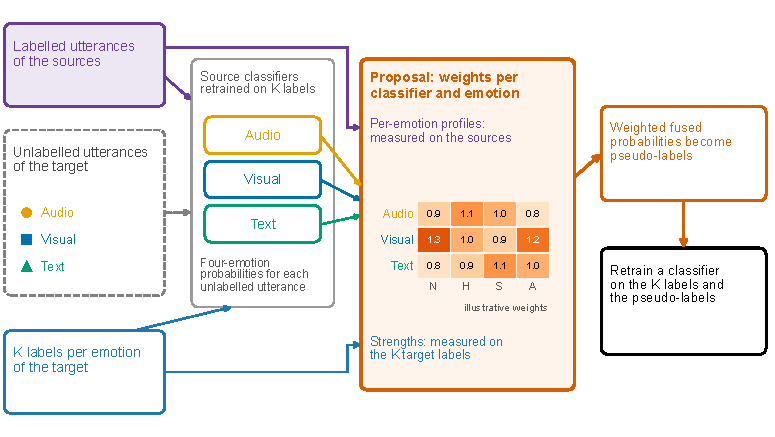
\includegraphics[width=\textwidth]{figures/fig_v4_overview_en.pdf}
\caption{The proposal combines the probabilities that the audio, visual and text classifiers (started from the source classifiers and retrained on the K target labels per emotion; Sect.~\ref{sec:distill}) assign to unlabelled target utterances with one weight per classifier and emotion, turns the fused probabilities into pseudo-labels, and retrains a classifier on them and the K labels per emotion. Each weight is built from the classifier's strength (its mean reliability over the four emotions), measured on the K target labels, and its per-emotion profile (how much its reliability for each emotion deviates from that mean), measured on the labelled source corpora. Weight values are illustrative}\label{fig:overview}
\end{figure}
